\Needspace{8\baselineskip}\originalchapter{2007 期末: 高压平衡与外 ballooning-kink}
题源: 22.615 Spring 2007 Final Part1与Part2. 两个公开文件分别含平衡8步、稳定6步; 按两道综合题计. 官方答案未取得, 以下为独立推导、可执行参考解及模型范围说明.
\begin{exercise}\label{ex:07-final-eq}
第一部分. 大长径比高beta排序, 圆核心半径a\ensuremath{{}^{\prime}}、近恒电流, 外围零电流无力等离子体, 再外真空至无穷. 核心/外区公开磁通为
\begin{align}
 \frac{\Psi_c}{a'^2B_0}&=\frac{r^2/a'^2-1+\nu'(r^3/a'^3-r/a')\cos\theta}{2q^{*\prime}},\\
 \frac{\Psi_o}{a'^2B_0}&=\frac{\ln(r/a')+\tfrac{\nu'}2(r/a'-a'/r)\cos\theta}{q^{*\prime}}.
\end{align}
选分离面内一条外磁面为真实等离子体边缘, 左半径a1、右a2, a=(a1+a2)/2. 输入\ensuremath{\zeta}1=a1/a>1, \ensuremath{\alpha}=a\ensuremath{{}^{\prime}}/a\ensuremath{\in}(0,1),轴$q_0=1.05$固定以避免内部m=n1锯齿. (1)求\ensuremath{\nu}\ensuremath{{}^{\prime}}(\ensuremath{\zeta}1,\ensuremath{\alpha}); (2)分离面触外边的关系; (3)画\ensuremath{\nu}\ensuremath{{}^{\prime}}/\ensuremath{\zeta}1及\ensuremath{\alpha}/\ensuremath{\zeta}1边界, 求1<\ensuremath{\zeta}crit<2; (4)写子程序求归一截面Ahat=A/(\ensuremath{\pi}a\ensuremath{{}^{2}}); (5)求\ensuremath{\nu}\ensuremath{{}^{\prime}}、$q^{*\prime}=2\pi a'^2B_0/(\mu_0R_0I)$、\ensuremath{\beta}t\ensuremath{{}^{\prime}}/\ensuremath{\epsilon}\ensuremath{{}^{\prime}}、$q_*=2AB_0/(\mu_0R_0I)$、\ensuremath{\beta}t/\ensuremath{\epsilon}、\ensuremath{\nu}=\ensuremath{\beta}tq*\ensuremath{{}^{2}}/\ensuremath{\epsilon}, \ensuremath{\beta}的平均分别核心圆和全外边区域, \ensuremath{\epsilon}\ensuremath{{}^{\prime}}=a\ensuremath{{}^{\prime}}/R0、\ensuremath{\epsilon}=a/R0; (6)画分离面约束在\ensuremath{\beta}t/\ensuremath{\epsilon}对1/q*边界; (7)外面缩到核心时另求边界并叠图形成闭允许域; (8)一般磁面q积分, 明算核心边qa\ensuremath{{}^{\prime}}并编程算qa. 不收录受限书本图, 以上公式与条件均在公开试卷印出.
\end{exercise}
\begin{solution}
\originalsection{外边界与两条平衡限制}
用s=r/a\ensuremath{{}^{\prime}}、L=\ensuremath{\zeta}1/\ensuremath{\alpha}、U=(2\ensuremath{-}\ensuremath{\zeta}1)/\ensuremath{\alpha}. 左\ensuremath{\theta}\ensuremath{\pi}、右\ensuremath{\theta}0在同一磁面, $\ln L-\nu'(L-L^{-1})/2=\ln U+\nu'(U-U^{-1})/2$, 故
\begin{equation}
 \nu'=\frac{\alpha\ln[\zeta_1/(2-\zeta_1)]}{1-\alpha^2/[\zeta_1(2-\zeta_1)]}.
\end{equation}
X点在\ensuremath{\theta}\ensuremath{\pi}, 外磁通径向导数零给\ensuremath{\nu}\ensuremath{{}^{\prime}}=2L/(L\ensuremath{{}^{2}}+1). 消\ensuremath{\nu}\ensuremath{{}^{\prime}}得到
\begin{equation}
 \alpha_{sep}^2=\frac{\zeta_1\{2-\zeta_1\ln[\zeta_1/(2-\zeta_1)]\}}
 {\ln[\zeta_1/(2-\zeta_1)]+2/(2-\zeta_1)}.
\end{equation}
需\ensuremath{\alpha}sep\ensuremath{{}^{2}}正, 端点$\zeta_{crit}$满足$\zeta_{crit}\ln[\zeta_{crit}/(2-\zeta_{crit})]=2$, 根1.56437658856. 分离面边界曲线如下, \ensuremath{\nu}\ensuremath{{}^{\prime}}由上两式计算.
\begin{center}\begin{tikzpicture}\begin{axis}[width=.67\textwidth,height=4.5cm,xlabel={$\zeta_1$},ylabel={分离面边界参数},xmin=1,xmax=1.57,ymin=0,ymax=1,legend style={font=\small}]
\addplot[thick,structurecolor] coordinates {(1.0000100,0.9999900) (1.0011387,0.9988613) (1.0022674,0.9977326) (1.0033961,0.9966038) (1.0045249,0.9954750) (1.0056536,0.9943462) (1.0067823,0.9932173) (1.0079110,0.9920884) (1.0090397,0.9909593) (1.0101684,0.9898302) (1.0112971,0.9887010) (1.0124258,0.9875716) (1.0135546,0.9864422) (1.0146833,0.9853126) (1.0158120,0.9841828) (1.0169407,0.9830529) (1.0180694,0.9819229) (1.0191981,0.9807926) (1.0203268,0.9796622) (1.0214555,0.9785316) (1.0225843,0.9774007) (1.0237130,0.9762696) (1.0248417,0.9751384) (1.0259704,0.9740068) (1.0270991,0.9728750) (1.0282278,0.9717430) (1.0293565,0.9706107) (1.0304853,0.9694780) (1.0316140,0.9683451) (1.0327427,0.9672119) (1.0338714,0.9660784) (1.0350001,0.9649446) (1.0361288,0.9638104) (1.0372575,0.9626759) (1.0383862,0.9615410) (1.0395150,0.9604057) (1.0406437,0.9592701) (1.0417724,0.9581341) (1.0429011,0.9569977) (1.0440298,0.9558609) (1.0451585,0.9547237) (1.0462872,0.9535860) (1.0474159,0.9524479) (1.0485447,0.9513094) (1.0496734,0.9501704) (1.0508021,0.9490310) (1.0519308,0.9478910) (1.0530595,0.9467506) (1.0541882,0.9456097) (1.0553169,0.9444683) (1.0564457,0.9433264) (1.0575744,0.9421839) (1.0587031,0.9410410) (1.0598318,0.9398974) (1.0609605,0.9387533) (1.0620892,0.9376087) (1.0632179,0.9364635) (1.0643466,0.9353177) (1.0654754,0.9341713) (1.0666041,0.9330243) (1.0677328,0.9318767) (1.0688615,0.9307285) (1.0699902,0.9295797) (1.0711189,0.9284302) (1.0722476,0.9272801) (1.0733763,0.9261293) (1.0745051,0.9249778) (1.0756338,0.9238257) (1.0767625,0.9226729) (1.0778912,0.9215194) (1.0790199,0.9203652) (1.0801486,0.9192103) (1.0812773,0.9180546) (1.0824060,0.9168982) (1.0835348,0.9157411) (1.0846635,0.9145832) (1.0857922,0.9134246) (1.0869209,0.9122652) (1.0880496,0.9111050) (1.0891783,0.9099440) (1.0903070,0.9087823) (1.0914358,0.9076197) (1.0925645,0.9064563) (1.0936932,0.9052921) (1.0948219,0.9041271) (1.0959506,0.9029612) (1.0970793,0.9017944) (1.0982080,0.9006268) (1.0993367,0.8994584) (1.1004655,0.8982890) (1.1015942,0.8971188) (1.1027229,0.8959476) (1.1038516,0.8947756) (1.1049803,0.8936026) (1.1061090,0.8924287) (1.1072377,0.8912539) (1.1083664,0.8900781) (1.1094952,0.8889014) (1.1106239,0.8877237) (1.1117526,0.8865451) (1.1128813,0.8853655) (1.1140100,0.8841848) (1.1151387,0.8830032) (1.1162674,0.8818206) (1.1173962,0.8806369) (1.1185249,0.8794523) (1.1196536,0.8782665) (1.1207823,0.8770798) (1.1219110,0.8758920) (1.1230397,0.8747031) (1.1241684,0.8735132) (1.1252971,0.8723221) (1.1264259,0.8711300) (1.1275546,0.8699368) (1.1286833,0.8687425) (1.1298120,0.8675470) (1.1309407,0.8663505) (1.1320694,0.8651528) (1.1331981,0.8639539) (1.1343268,0.8627539) (1.1354556,0.8615527) (1.1365843,0.8603504) (1.1377130,0.8591469) (1.1388417,0.8579421) (1.1399704,0.8567362) (1.1410991,0.8555291) (1.1422278,0.8543207) (1.1433566,0.8531112) (1.1444853,0.8519003) (1.1456140,0.8506883) (1.1467427,0.8494749) (1.1478714,0.8482603) (1.1490001,0.8470445) (1.1501288,0.8458273) (1.1512575,0.8446089) (1.1523863,0.8433891) (1.1535150,0.8421680) (1.1546437,0.8409457) (1.1557724,0.8397219) (1.1569011,0.8384969) (1.1580298,0.8372704) (1.1591585,0.8360427) (1.1602872,0.8348135) (1.1614160,0.8335830) (1.1625447,0.8323510) (1.1636734,0.8311177) (1.1648021,0.8298830) (1.1659308,0.8286468) (1.1670595,0.8274092) (1.1681882,0.8261702) (1.1693170,0.8249297) (1.1704457,0.8236878) (1.1715744,0.8224444) (1.1727031,0.8211995) (1.1738318,0.8199531) (1.1749605,0.8187053) (1.1760892,0.8174559) (1.1772179,0.8162050) (1.1783467,0.8149526) (1.1794754,0.8136986) (1.1806041,0.8124431) (1.1817328,0.8111860) (1.1828615,0.8099274) (1.1839902,0.8086672) (1.1851189,0.8074054) (1.1862476,0.8061420) (1.1873764,0.8048770) (1.1885051,0.8036103) (1.1896338,0.8023421) (1.1907625,0.8010722) (1.1918912,0.7998006) (1.1930199,0.7985274) (1.1941486,0.7972525) (1.1952773,0.7959759) (1.1964061,0.7946977) (1.1975348,0.7934177) (1.1986635,0.7921360) (1.1997922,0.7908526) (1.2009209,0.7895674) (1.2020496,0.7882805) (1.2031783,0.7869919) (1.2043071,0.7857015) (1.2054358,0.7844093) (1.2065645,0.7831153) (1.2076932,0.7818195) (1.2088219,0.7805219) (1.2099506,0.7792225) (1.2110793,0.7779212) (1.2122080,0.7766181) (1.2133368,0.7753131) (1.2144655,0.7740063) (1.2155942,0.7726976) (1.2167229,0.7713870) (1.2178516,0.7700744) (1.2189803,0.7687600) (1.2201090,0.7674437) (1.2212377,0.7661254) (1.2223665,0.7648051) (1.2234952,0.7634829) (1.2246239,0.7621587) (1.2257526,0.7608326) (1.2268813,0.7595044) (1.2280100,0.7581742) (1.2291387,0.7568421) (1.2302675,0.7555078) (1.2313962,0.7541716) (1.2325249,0.7528332) (1.2336536,0.7514928) (1.2347823,0.7501503) (1.2359110,0.7488057) (1.2370397,0.7474590) (1.2381684,0.7461102) (1.2392972,0.7447593) (1.2404259,0.7434062) (1.2415546,0.7420509) (1.2426833,0.7406935) (1.2438120,0.7393339) (1.2449407,0.7379721) (1.2460694,0.7366080) (1.2471981,0.7352418) (1.2483269,0.7338733) (1.2494556,0.7325025) (1.2505843,0.7311295) (1.2517130,0.7297542) (1.2528417,0.7283766) (1.2539704,0.7269967) (1.2550991,0.7256145) (1.2562279,0.7242299) (1.2573566,0.7228430) (1.2584853,0.7214538) (1.2596140,0.7200621) (1.2607427,0.7186681) (1.2618714,0.7172716) (1.2630001,0.7158727) (1.2641288,0.7144714) (1.2652576,0.7130677) (1.2663863,0.7116614) (1.2675150,0.7102527) (1.2686437,0.7088415) (1.2697724,0.7074278) (1.2709011,0.7060115) (1.2720298,0.7045927) (1.2731585,0.7031713) (1.2742873,0.7017474) (1.2754160,0.7003209) (1.2765447,0.6988917) (1.2776734,0.6974600) (1.2788021,0.6960256) (1.2799308,0.6945885) (1.2810595,0.6931488) (1.2821882,0.6917063) (1.2833170,0.6902612) (1.2844457,0.6888134) (1.2855744,0.6873628) (1.2867031,0.6859094) (1.2878318,0.6844533) (1.2889605,0.6829944) (1.2900892,0.6815326) (1.2912180,0.6800681) (1.2923467,0.6786006) (1.2934754,0.6771304) (1.2946041,0.6756572) (1.2957328,0.6741811) (1.2968615,0.6727022) (1.2979902,0.6712202) (1.2991189,0.6697354) (1.3002477,0.6682475) (1.3013764,0.6667566) (1.3025051,0.6652628) (1.3036338,0.6637658) (1.3047625,0.6622659) (1.3058912,0.6607628) (1.3070199,0.6592567) (1.3081486,0.6577474) (1.3092774,0.6562350) (1.3104061,0.6547194) (1.3115348,0.6532007) (1.3126635,0.6516788) (1.3137922,0.6501536) (1.3149209,0.6486252) (1.3160496,0.6470935) (1.3171784,0.6455585) (1.3183071,0.6440202) (1.3194358,0.6424786) (1.3205645,0.6409337) (1.3216932,0.6393853) (1.3228219,0.6378335) (1.3239506,0.6362784) (1.3250793,0.6347197) (1.3262081,0.6331576) (1.3273368,0.6315920) (1.3284655,0.6300228) (1.3295942,0.6284502) (1.3307229,0.6268739) (1.3318516,0.6252940) (1.3329803,0.6237105) (1.3341090,0.6221234) (1.3352378,0.6205326) (1.3363665,0.6189380) (1.3374952,0.6173398) (1.3386239,0.6157378) (1.3397526,0.6141320) (1.3408813,0.6125223) (1.3420100,0.6109089) (1.3431388,0.6092915) (1.3442675,0.6076703) (1.3453962,0.6060451) (1.3465249,0.6044160) (1.3476536,0.6027829) (1.3487823,0.6011457) (1.3499110,0.5995046) (1.3510397,0.5978593) (1.3521685,0.5962099) (1.3532972,0.5945564) (1.3544259,0.5928987) (1.3555546,0.5912368) (1.3566833,0.5895706) (1.3578120,0.5879002) (1.3589407,0.5862254) (1.3600694,0.5845463) (1.3611982,0.5828628) (1.3623269,0.5811750) (1.3634556,0.5794826) (1.3645843,0.5777858) (1.3657130,0.5760844) (1.3668417,0.5743785) (1.3679704,0.5726680) (1.3690992,0.5709529) (1.3702279,0.5692330) (1.3713566,0.5675085) (1.3724853,0.5657792) (1.3736140,0.5640451) (1.3747427,0.5623062) (1.3758714,0.5605623) (1.3770001,0.5588136) (1.3781289,0.5570599) (1.3792576,0.5553012) (1.3803863,0.5535374) (1.3815150,0.5517686) (1.3826437,0.5499946) (1.3837724,0.5482154) (1.3849011,0.5464309) (1.3860298,0.5446412) (1.3871586,0.5428462) (1.3882873,0.5410458) (1.3894160,0.5392399) (1.3905447,0.5374286) (1.3916734,0.5356117) (1.3928021,0.5337892) (1.3939308,0.5319611) (1.3950596,0.5301273) (1.3961883,0.5282878) (1.3973170,0.5264425) (1.3984457,0.5245913) (1.3995744,0.5227341) (1.4007031,0.5208710) (1.4018318,0.5190019) (1.4029605,0.5171267) (1.4040893,0.5152453) (1.4052180,0.5133576) (1.4063467,0.5114637) (1.4074754,0.5095635) (1.4086041,0.5076568) (1.4097328,0.5057436) (1.4108615,0.5038239) (1.4119902,0.5018976) (1.4131190,0.4999646) (1.4142477,0.4980248) (1.4153764,0.4960781) (1.4165051,0.4941245) (1.4176338,0.4921640) (1.4187625,0.4901964) (1.4198912,0.4882216) (1.4210199,0.4862396) (1.4221487,0.4842502) (1.4232774,0.4822535) (1.4244061,0.4802493) (1.4255348,0.4782375) (1.4266635,0.4762181) (1.4277922,0.4741908) (1.4289209,0.4721558) (1.4300497,0.4701128) (1.4311784,0.4680617) (1.4323071,0.4660025) (1.4334358,0.4639351) (1.4345645,0.4618593) (1.4356932,0.4597751) (1.4368219,0.4576823) (1.4379506,0.4555808) (1.4390794,0.4534706) (1.4402081,0.4513514) (1.4413368,0.4492232) (1.4424655,0.4470859) (1.4435942,0.4449393) (1.4447229,0.4427833) (1.4458516,0.4406178) (1.4469803,0.4384426) (1.4481091,0.4362577) (1.4492378,0.4340628) (1.4503665,0.4318578) (1.4514952,0.4296426) (1.4526239,0.4274171) (1.4537526,0.4251810) (1.4548813,0.4229342) (1.4560101,0.4206766) (1.4571388,0.4184079) (1.4582675,0.4161281) (1.4593962,0.4138369) (1.4605249,0.4115342) (1.4616536,0.4092197) (1.4627823,0.4068934) (1.4639110,0.4045549) (1.4650398,0.4022041) (1.4661685,0.3998407) (1.4672972,0.3974647) (1.4684259,0.3950756) (1.4695546,0.3926734) (1.4706833,0.3902578) (1.4718120,0.3878285) (1.4729407,0.3853854) (1.4740695,0.3829280) (1.4751982,0.3804563) (1.4763269,0.3779698) (1.4774556,0.3754684) (1.4785843,0.3729517) (1.4797130,0.3704195) (1.4808417,0.3678713) (1.4819705,0.3653070) (1.4830992,0.3627262) (1.4842279,0.3601285) (1.4853566,0.3575136) (1.4864853,0.3548811) (1.4876140,0.3522306) (1.4887427,0.3495618) (1.4898714,0.3468742) (1.4910002,0.3441673) (1.4921289,0.3414409) (1.4932576,0.3386943) (1.4943863,0.3359272) (1.4955150,0.3331389) (1.4966437,0.3303291) (1.4977724,0.3274971) (1.4989011,0.3246425) (1.5000299,0.3217645) (1.5011586,0.3188626) (1.5022873,0.3159362) (1.5034160,0.3129845) (1.5045447,0.3100069) (1.5056734,0.3070027) (1.5068021,0.3039710) (1.5079308,0.3009110) (1.5090596,0.2978220) (1.5101883,0.2947029) (1.5113170,0.2915529) (1.5124457,0.2883710) (1.5135744,0.2851560) (1.5147031,0.2819070) (1.5158318,0.2786227) (1.5169606,0.2753019) (1.5180893,0.2719432) (1.5192180,0.2685453) (1.5203467,0.2651067) (1.5214754,0.2616258) (1.5226041,0.2581008) (1.5237328,0.2545301) (1.5248615,0.2509117) (1.5259903,0.2472434) (1.5271190,0.2435232) (1.5282477,0.2397485) (1.5293764,0.2359168) (1.5305051,0.2320252) (1.5316338,0.2280709) (1.5327625,0.2240504) (1.5338912,0.2199601) (1.5350200,0.2157962) (1.5361487,0.2115542) (1.5372774,0.2072295) (1.5384061,0.2028168) (1.5395348,0.1983102) (1.5406635,0.1937032) (1.5417922,0.1889885) (1.5429210,0.1841579) (1.5440497,0.1792021) (1.5451784,0.1741103) (1.5463071,0.1688703) (1.5474358,0.1634679) (1.5485645,0.1578866) (1.5496932,0.1521065) (1.5508219,0.1461043) (1.5519507,0.1398512) (1.5530794,0.1333122) (1.5542081,0.1264429) (1.5553368,0.1191863) (1.5564655,0.1114668) (1.5575942,0.1031806) (1.5587229,0.0941783) (1.5598516,0.0842309) (1.5609804,0.0729526) (1.5621091,0.0595929) (1.5632378,0.0422202) (1.5643665,0.0039727)};\addlegendentry{$\alpha_{sep}$}
\addplot[thick,dashed] coordinates {(1.0000100,1.0000000) (1.0011387,0.9999974) (1.0022674,0.9999897) (1.0033961,0.9999769) (1.0045249,0.9999591) (1.0056536,0.9999361) (1.0067823,0.9999080) (1.0079110,0.9998748) (1.0090397,0.9998366) (1.0101684,0.9997932) (1.0112971,0.9997447) (1.0124258,0.9996912) (1.0135546,0.9996325) (1.0146833,0.9995688) (1.0158120,0.9994999) (1.0169407,0.9994260) (1.0180694,0.9993469) (1.0191981,0.9992628) (1.0203268,0.9991735) (1.0214555,0.9990792) (1.0225843,0.9989797) (1.0237130,0.9988752) (1.0248417,0.9987655) (1.0259704,0.9986508) (1.0270991,0.9985309) (1.0282278,0.9984060) (1.0293565,0.9982759) (1.0304853,0.9981407) (1.0316140,0.9980004) (1.0327427,0.9978551) (1.0338714,0.9977046) (1.0350001,0.9975490) (1.0361288,0.9973883) (1.0372575,0.9972225) (1.0383862,0.9970515) (1.0395150,0.9968755) (1.0406437,0.9966944) (1.0417724,0.9965081) (1.0429011,0.9963167) (1.0440298,0.9961202) (1.0451585,0.9959186) (1.0462872,0.9957119) (1.0474159,0.9955001) (1.0485447,0.9952831) (1.0496734,0.9950610) (1.0508021,0.9948338) (1.0519308,0.9946015) (1.0530595,0.9943641) (1.0541882,0.9941215) (1.0553169,0.9938738) (1.0564457,0.9936210) (1.0575744,0.9933630) (1.0587031,0.9930999) (1.0598318,0.9928317) (1.0609605,0.9925584) (1.0620892,0.9922799) (1.0632179,0.9919963) (1.0643466,0.9917075) (1.0654754,0.9914136) (1.0666041,0.9911146) (1.0677328,0.9908104) (1.0688615,0.9905011) (1.0699902,0.9901866) (1.0711189,0.9898670) (1.0722476,0.9895422) (1.0733763,0.9892123) (1.0745051,0.9888772) (1.0756338,0.9885370) (1.0767625,0.9881916) (1.0778912,0.9878411) (1.0790199,0.9874854) (1.0801486,0.9871245) (1.0812773,0.9867585) (1.0824060,0.9863873) (1.0835348,0.9860110) (1.0846635,0.9856295) (1.0857922,0.9852428) (1.0869209,0.9848509) (1.0880496,0.9844539) (1.0891783,0.9840516) (1.0903070,0.9836442) (1.0914358,0.9832316) (1.0925645,0.9828139) (1.0936932,0.9823909) (1.0948219,0.9819628) (1.0959506,0.9815294) (1.0970793,0.9810909) (1.0982080,0.9806472) (1.0993367,0.9801982) (1.1004655,0.9797441) (1.1015942,0.9792848) (1.1027229,0.9788202) (1.1038516,0.9783505) (1.1049803,0.9778755) (1.1061090,0.9773954) (1.1072377,0.9769100) (1.1083664,0.9764193) (1.1094952,0.9759235) (1.1106239,0.9754225) (1.1117526,0.9749162) (1.1128813,0.9744046) (1.1140100,0.9738879) (1.1151387,0.9733659) (1.1162674,0.9728387) (1.1173962,0.9723062) (1.1185249,0.9717685) (1.1196536,0.9712255) (1.1207823,0.9706773) (1.1219110,0.9701238) (1.1230397,0.9695650) (1.1241684,0.9690010) (1.1252971,0.9684318) (1.1264259,0.9678572) (1.1275546,0.9672774) (1.1286833,0.9666923) (1.1298120,0.9661020) (1.1309407,0.9655063) (1.1320694,0.9649054) (1.1331981,0.9642992) (1.1343268,0.9636877) (1.1354556,0.9630709) (1.1365843,0.9624487) (1.1377130,0.9618213) (1.1388417,0.9611886) (1.1399704,0.9605506) (1.1410991,0.9599072) (1.1422278,0.9592585) (1.1433566,0.9586045) (1.1444853,0.9579452) (1.1456140,0.9572805) (1.1467427,0.9566105) (1.1478714,0.9559352) (1.1490001,0.9552545) (1.1501288,0.9545685) (1.1512575,0.9538771) (1.1523863,0.9531804) (1.1535150,0.9524783) (1.1546437,0.9517708) (1.1557724,0.9510580) (1.1569011,0.9503397) (1.1580298,0.9496162) (1.1591585,0.9488872) (1.1602872,0.9481528) (1.1614160,0.9474130) (1.1625447,0.9466679) (1.1636734,0.9459173) (1.1648021,0.9451613) (1.1659308,0.9443999) (1.1670595,0.9436331) (1.1681882,0.9428609) (1.1693170,0.9420833) (1.1704457,0.9413002) (1.1715744,0.9405116) (1.1727031,0.9397177) (1.1738318,0.9389182) (1.1749605,0.9381133) (1.1760892,0.9373030) (1.1772179,0.9364872) (1.1783467,0.9356659) (1.1794754,0.9348392) (1.1806041,0.9340069) (1.1817328,0.9331692) (1.1828615,0.9323260) (1.1839902,0.9314773) (1.1851189,0.9306230) (1.1862476,0.9297633) (1.1873764,0.9288980) (1.1885051,0.9280272) (1.1896338,0.9271509) (1.1907625,0.9262691) (1.1918912,0.9253817) (1.1930199,0.9244887) (1.1941486,0.9235902) (1.1952773,0.9226862) (1.1964061,0.9217765) (1.1975348,0.9208613) (1.1986635,0.9199406) (1.1997922,0.9190142) (1.2009209,0.9180822) (1.2020496,0.9171446) (1.2031783,0.9162014) (1.2043071,0.9152526) (1.2054358,0.9142982) (1.2065645,0.9133381) (1.2076932,0.9123724) (1.2088219,0.9114011) (1.2099506,0.9104241) (1.2110793,0.9094414) (1.2122080,0.9084531) (1.2133368,0.9074591) (1.2144655,0.9064594) (1.2155942,0.9054540) (1.2167229,0.9044430) (1.2178516,0.9034262) (1.2189803,0.9024037) (1.2201090,0.9013754) (1.2212377,0.9003415) (1.2223665,0.8993018) (1.2234952,0.8982563) (1.2246239,0.8972051) (1.2257526,0.8961481) (1.2268813,0.8950854) (1.2280100,0.8940168) (1.2291387,0.8929425) (1.2302675,0.8918624) (1.2313962,0.8907764) (1.2325249,0.8896846) (1.2336536,0.8885870) (1.2347823,0.8874836) (1.2359110,0.8863743) (1.2370397,0.8852592) (1.2381684,0.8841382) (1.2392972,0.8830113) (1.2404259,0.8818785) (1.2415546,0.8807398) (1.2426833,0.8795952) (1.2438120,0.8784447) (1.2449407,0.8772883) (1.2460694,0.8761259) (1.2471981,0.8749576) (1.2483269,0.8737833) (1.2494556,0.8726031) (1.2505843,0.8714168) (1.2517130,0.8702246) (1.2528417,0.8690264) (1.2539704,0.8678221) (1.2550991,0.8666118) (1.2562279,0.8653955) (1.2573566,0.8641731) (1.2584853,0.8629447) (1.2596140,0.8617102) (1.2607427,0.8604696) (1.2618714,0.8592229) (1.2630001,0.8579701) (1.2641288,0.8567111) (1.2652576,0.8554461) (1.2663863,0.8541749) (1.2675150,0.8528975) (1.2686437,0.8516139) (1.2697724,0.8503242) (1.2709011,0.8490282) (1.2720298,0.8477261) (1.2731585,0.8464177) (1.2742873,0.8451030) (1.2754160,0.8437821) (1.2765447,0.8424549) (1.2776734,0.8411215) (1.2788021,0.8397817) (1.2799308,0.8384357) (1.2810595,0.8370833) (1.2821882,0.8357245) (1.2833170,0.8343594) (1.2844457,0.8329879) (1.2855744,0.8316100) (1.2867031,0.8302258) (1.2878318,0.8288350) (1.2889605,0.8274379) (1.2900892,0.8260343) (1.2912180,0.8246242) (1.2923467,0.8232076) (1.2934754,0.8217846) (1.2946041,0.8203550) (1.2957328,0.8189188) (1.2968615,0.8174761) (1.2979902,0.8160269) (1.2991189,0.8145710) (1.3002477,0.8131085) (1.3013764,0.8116394) (1.3025051,0.8101637) (1.3036338,0.8086812) (1.3047625,0.8071921) (1.3058912,0.8056963) (1.3070199,0.8041937) (1.3081486,0.8026844) (1.3092774,0.8011684) (1.3104061,0.7996455) (1.3115348,0.7981159) (1.3126635,0.7965794) (1.3137922,0.7950361) (1.3149209,0.7934858) (1.3160496,0.7919287) (1.3171784,0.7903647) (1.3183071,0.7887938) (1.3194358,0.7872159) (1.3205645,0.7856310) (1.3216932,0.7840391) (1.3228219,0.7824401) (1.3239506,0.7808341) (1.3250793,0.7792211) (1.3262081,0.7776009) (1.3273368,0.7759736) (1.3284655,0.7743392) (1.3295942,0.7726976) (1.3307229,0.7710487) (1.3318516,0.7693927) (1.3329803,0.7677294) (1.3341090,0.7660588) (1.3352378,0.7643809) (1.3363665,0.7626957) (1.3374952,0.7610030) (1.3386239,0.7593031) (1.3397526,0.7575956) (1.3408813,0.7558808) (1.3420100,0.7541584) (1.3431388,0.7524286) (1.3442675,0.7506911) (1.3453962,0.7489462) (1.3465249,0.7471936) (1.3476536,0.7454334) (1.3487823,0.7436655) (1.3499110,0.7418899) (1.3510397,0.7401066) (1.3521685,0.7383155) (1.3532972,0.7365166) (1.3544259,0.7347099) (1.3555546,0.7328953) (1.3566833,0.7310728) (1.3578120,0.7292424) (1.3589407,0.7274040) (1.3600694,0.7255575) (1.3611982,0.7237030) (1.3623269,0.7218404) (1.3634556,0.7199697) (1.3645843,0.7180908) (1.3657130,0.7162037) (1.3668417,0.7143084) (1.3679704,0.7124047) (1.3690992,0.7104927) (1.3702279,0.7085724) (1.3713566,0.7066436) (1.3724853,0.7047063) (1.3736140,0.7027605) (1.3747427,0.7008062) (1.3758714,0.6988433) (1.3770001,0.6968717) (1.3781289,0.6948914) (1.3792576,0.6929023) (1.3803863,0.6909045) (1.3815150,0.6888978) (1.3826437,0.6868822) (1.3837724,0.6848577) (1.3849011,0.6828242) (1.3860298,0.6807816) (1.3871586,0.6787299) (1.3882873,0.6766690) (1.3894160,0.6745989) (1.3905447,0.6725195) (1.3916734,0.6704307) (1.3928021,0.6683326) (1.3939308,0.6662250) (1.3950596,0.6641079) (1.3961883,0.6619812) (1.3973170,0.6598448) (1.3984457,0.6576987) (1.3995744,0.6555428) (1.4007031,0.6533771) (1.4018318,0.6512015) (1.4029605,0.6490158) (1.4040893,0.6468202) (1.4052180,0.6446143) (1.4063467,0.6423983) (1.4074754,0.6401720) (1.4086041,0.6379353) (1.4097328,0.6356881) (1.4108615,0.6334305) (1.4119902,0.6311622) (1.4131190,0.6288833) (1.4142477,0.6265935) (1.4153764,0.6242930) (1.4165051,0.6219814) (1.4176338,0.6196589) (1.4187625,0.6173252) (1.4198912,0.6149802) (1.4210199,0.6126240) (1.4221487,0.6102563) (1.4232774,0.6078772) (1.4244061,0.6054863) (1.4255348,0.6030838) (1.4266635,0.6006694) (1.4277922,0.5982431) (1.4289209,0.5958048) (1.4300497,0.5933542) (1.4311784,0.5908914) (1.4323071,0.5884162) (1.4334358,0.5859285) (1.4345645,0.5834281) (1.4356932,0.5809149) (1.4368219,0.5783888) (1.4379506,0.5758497) (1.4390794,0.5732974) (1.4402081,0.5707318) (1.4413368,0.5681527) (1.4424655,0.5655600) (1.4435942,0.5629536) (1.4447229,0.5603332) (1.4458516,0.5576988) (1.4469803,0.5550501) (1.4481091,0.5523871) (1.4492378,0.5497095) (1.4503665,0.5470171) (1.4514952,0.5443098) (1.4526239,0.5415874) (1.4537526,0.5388498) (1.4548813,0.5360966) (1.4560101,0.5333277) (1.4571388,0.5305430) (1.4582675,0.5277422) (1.4593962,0.5249250) (1.4605249,0.5220914) (1.4616536,0.5192409) (1.4627823,0.5163735) (1.4639110,0.5134888) (1.4650398,0.5105866) (1.4661685,0.5076667) (1.4672972,0.5047288) (1.4684259,0.5017726) (1.4695546,0.4987979) (1.4706833,0.4958043) (1.4718120,0.4927915) (1.4729407,0.4897594) (1.4740695,0.4867074) (1.4751982,0.4836354) (1.4763269,0.4805429) (1.4774556,0.4774297) (1.4785843,0.4742953) (1.4797130,0.4711395) (1.4808417,0.4679617) (1.4819705,0.4647616) (1.4830992,0.4615388) (1.4842279,0.4582929) (1.4853566,0.4550235) (1.4864853,0.4517299) (1.4876140,0.4484119) (1.4887427,0.4450689) (1.4898714,0.4417003) (1.4910002,0.4383057) (1.4921289,0.4348845) (1.4932576,0.4314361) (1.4943863,0.4279599) (1.4955150,0.4244553) (1.4966437,0.4209216) (1.4977724,0.4173582) (1.4989011,0.4137643) (1.5000299,0.4101392) (1.5011586,0.4064822) (1.5022873,0.4027924) (1.5034160,0.3990689) (1.5045447,0.3953109) (1.5056734,0.3915175) (1.5068021,0.3876877) (1.5079308,0.3838204) (1.5090596,0.3799146) (1.5101883,0.3759691) (1.5113170,0.3719828) (1.5124457,0.3679543) (1.5135744,0.3638825) (1.5147031,0.3597657) (1.5158318,0.3556027) (1.5169606,0.3513917) (1.5180893,0.3471311) (1.5192180,0.3428192) (1.5203467,0.3384541) (1.5214754,0.3340337) (1.5226041,0.3295559) (1.5237328,0.3250184) (1.5248615,0.3204188) (1.5259903,0.3157544) (1.5271190,0.3110224) (1.5282477,0.3062198) (1.5293764,0.3013432) (1.5305051,0.2963890) (1.5316338,0.2913536) (1.5327625,0.2862325) (1.5338912,0.2810213) (1.5350200,0.2757149) (1.5361487,0.2703079) (1.5372774,0.2647941) (1.5384061,0.2591669) (1.5395348,0.2534187) (1.5406635,0.2475413) (1.5417922,0.2415254) (1.5429210,0.2353604) (1.5440497,0.2290345) (1.5451784,0.2225340) (1.5463071,0.2158433) (1.5474358,0.2089442) (1.5485645,0.2018155) (1.5496932,0.1944322) (1.5508219,0.1867640) (1.5519507,0.1787747) (1.5530794,0.1704191) (1.5542081,0.1616406) (1.5553368,0.1523663) (1.5564655,0.1424998) (1.5575942,0.1319083) (1.5587229,0.1204008) (1.5598516,0.1076846) (1.5609804,0.0932666) (1.5621091,0.0761872) (1.5632378,0.0539770) (1.5643665,0.0050790)};\addlegendentry{$\nu_{sep}^\prime$}
\end{axis}\end{tikzpicture}\end{center}

可取1<\ensuremath{\zeta}1<\ensuremath{\zeta}crit,0<\ensuremath{\alpha}<\ensuremath{\alpha}sep; 等号分离面qa发散, 不是普通有限闭面. 另一限制外面=核心即$\alpha=1$, 应取解析极限而非将\ensuremath{\zeta}1=1代入0/0.

\originalsection{面积与 q 的实际积分}
定义\ensuremath{\chi}(s,\ensuremath{\theta})=lns+\ensuremath{\nu}\ensuremath{{}^{\prime}}(s\ensuremath{-}1/s)cos\ensuremath{\theta}/2. 外面满足$\chi(s_b,\theta)=\chi(L,\pi)$. 每角在[1,L]二分取最内侧闭合根, 避免X点外分支, 得 $\widehat A=\alpha^2\int s_b^2\dd\theta/(2\pi)$. 一般高beta q为 $q= B_0\oint dl_p/(2\pi R_0B_p)$; 按磁面径向微分也可用 $q=(B_0/(2\pi))\dd A/\dd\Psi$ 的一致归一, 正负通量方向取正绕行比. 核心磁轴从x方向二次方程得 $s_{axis}=(\eta-1)/(3\nu')$, $\eta=\sqrt{1+3\nu^{\prime2}}$; 磁通Hessian主值比给
\begin{equation}
 q'=q^{*\prime}=q_0\sqrt{\frac{\eta(2+\eta)}3},\quad
 q_{a'}=\frac{q'}{\sqrt{1-\nu'^2}},\quad
 q_a=\frac{q'}{2\pi}\int_0^{2\pi}\frac{s_b^2\dd\theta}{1+\nu'(s_b+s_b^{-1})\cos\theta/2}.
\end{equation}
$\nu^{\prime}=0$轴值连续取q\ensuremath{{}^{\prime}}=q0. 外无力区压强与核心边相同为0, 所以总压力积分等于核心压力积分, 而平均面积改变. 因此
\begin{align}
 \frac{\beta_t'}{\epsilon'}&=\frac{\nu'}{q'^2},\qquad
 q_*=q'\frac{\widehat A}{\alpha^2},\\
 \frac{\beta_t}{\epsilon}&=\frac{\nu'\alpha^3}{q'^2\widehat A},\qquad
 \nu=\frac{\beta_tq_*^2}{\epsilon}=\nu'\frac{\widehat A}{\alpha}.
\end{align}
$\alpha=1$给q*=q\ensuremath{{}^{\prime}},\ensuremath{\beta}t/\ensuremath{\epsilon}=\ensuremath{\nu}\ensuremath{{}^{\prime}}/q\ensuremath{{}^{\prime}}\ensuremath{{}^{2}}, 是另一平衡边界. 后面的稳定空间图同时包含两边界.

\originalsection{可复算样例}
取$\zeta_1=1.1,\alpha=.6$, 实际积分为
\begin{align}
 \nu'&=.1892037986,& \widehat A&=.9783468345,& q'&=1.0864752481,\\
 q_*&=2.9526378327,&q_{a'}&=1.1064603107,&q_a&=3.1066847943,\\
 \beta_t/\epsilon&=.0353875980.&&&&
\end{align}
 用128至1024 Gauss角点比较四个非奇异样例, 面积/q/最低能量在约 $10^{-12}$内一致. \ensuremath{\theta}\ensuremath{\pi}处分段以解析分离面附近尖峰; 精确分离面上只画允许域边界, 不报有限qa.
\begin{center}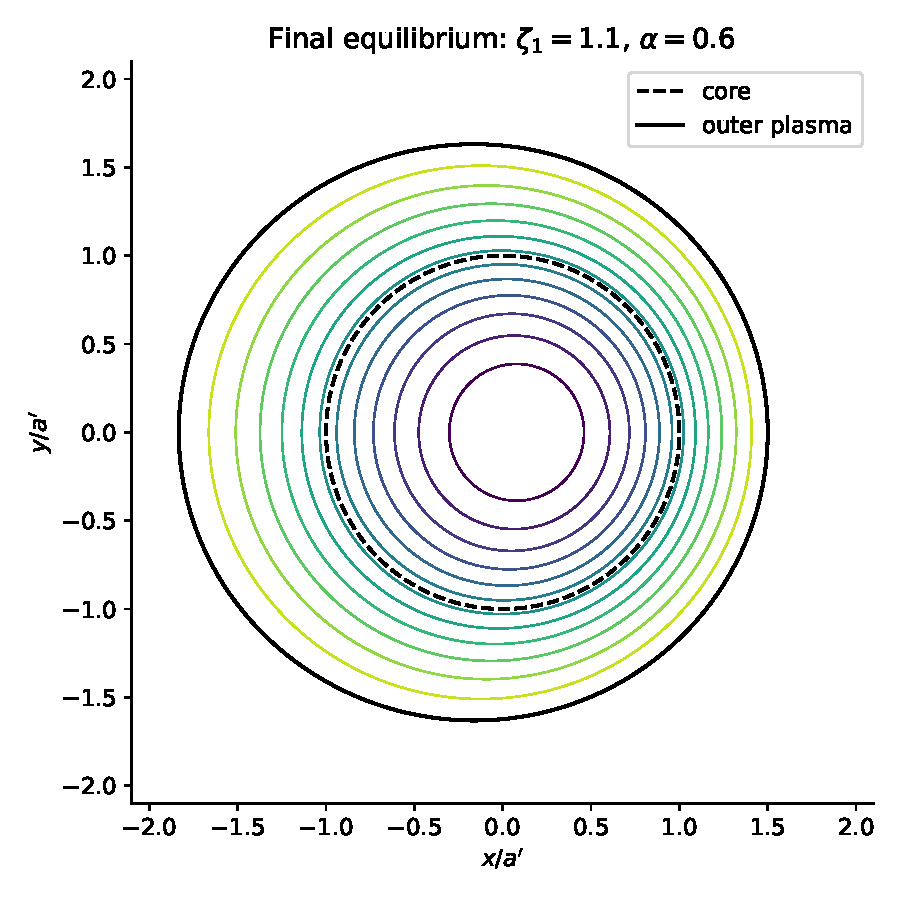
\includegraphics[width=.65\textwidth]{figures/final_flux.pdf}\end{center}
图为实际核心及外闭磁面; 内外中平面距离不等, a按左右半径均值定义, 不把圆核心面积替代真实外面积.
\end{solution}
\begin{exercise}\label{ex:07-final-stable}
第二部分. $n=1$最危险外ballooning-kink, 用高beta排序的能量原理. 原件说明最不稳可取不可压, 磁压缩最高阶正能需div\ensuremath{\xi}\ensuremath{\perp}0=0, 一阶校正取div\ensuremath{\xi}\ensuremath{\perp}1=\ensuremath{-}2\ensuremath{\xi}\ensuremath{\perp}0·\ensuremath{\kappa}以消正磁压缩. (1)核查各项阶数, 以二维\ensuremath{\xi}r/\ensuremath{\xi}\ensuremath{\theta},Qr/Q\ensuremath{\theta}写剩余能量; 由核心\ensuremath{\Psi}求Br/B\ensuremath{\theta}, Br须用试卷勘误正号. (2)对m\ensuremath{\ge}2取 $\xi_r=c_{m-1}\rho^{m-2}\e^{\ii(m-1)\theta}+c_m\rho^{m-1}\e^{\ii m\theta}+c_{m+1}\rho^m\e^{\ii(m+1)\theta}$、\ensuremath{\rho}=r/a\ensuremath{{}^{\prime}}, 求\ensuremath{\xi}\ensuremath{\theta},Qr,Q\ensuremath{\theta}. (3)算\ensuremath{\delta}WF=c†WFc, 实对称3\ensuremath{\times}3. (4)先把核心外当真空$\mathbf B_1=\nabla\Phi,\nabla^2\Phi=0$, 求核心界面条件、\ensuremath{\Phi}有几谐波; 每\ensuremath{\ell}谐波有圆同心理想壁b\ensuremath{\ell}, 求壁条件. (5)解\ensuremath{\Phi}、不用Bessel、算WV. (6)扫\ensuremath{\zeta}1/\ensuremath{\alpha}及几个m, W=WF+WV最低特征值零求边界, 叠平衡域, 找最高稳定\ensuremath{\beta}t/\ensuremath{\epsilon}、q*, 比Troyon.

等效壁按题规定: qa\ensuremath{{}^{\prime}}<qa<\ensuremath{\ell}取无穷; qa\ensuremath{{}^{\prime}}<\ensuremath{\ell}<qa则二次q(r)=qa\ensuremath{{}^{\prime}}+(qa\ensuremath{-}qa\ensuremath{{}^{\prime}})(r\ensuremath{{}^{2}}\ensuremath{-}a\ensuremath{{}^{\prime}}\ensuremath{{}^{2}})/(a\ensuremath{{}^{2}}\ensuremath{-}a\ensuremath{{}^{\prime}}\ensuremath{{}^{2}}), $b_\ell^2=a'^2+(a^2-a'^2)(\ell-q_{a'})/(q_a-q_{a'})$; \ensuremath{\ell}<qa\ensuremath{{}^{\prime}}<qa仍取无穷且不改核心试函数. 这是指定的外无力区近似, 不是真实外区全MHD求解.
\end{exercise}
\begin{solution}
\originalsection{阶数、方向和流体能量}
Bp/B0=O(\ensuremath{\epsilon}), \ensuremath{\xi}\ensuremath{\perp}尺度a\ensuremath{{}^{\prime}}, 未约束的磁压缩 $B_0^2(\nabla\cdot\xi_\perp)^2$最大. 线弯曲与压强-曲率项小\ensuremath{\epsilon}\ensuremath{{}^{2}}, 要发现负能先极小化最高阶正项; 题给两阶散度条件消掉它. 保留章\ref{ch:energy}的SI量纲, 将R--Z极角与环向的左手关系改用右手z=\ensuremath{-}R0\ensuremath{\phi}, Bz=\ensuremath{-}B0, 模态e$^{i(j\ensuremath{\theta}+z/R_0)}$. 这样沿场相位仍j/q\ensuremath{-}1. 磁场以K=B0a\ensuremath{{}^{\prime}}/R0归一, r以下无量纲\ensuremath{\rho}:
\begin{equation}
 \widehat B_r=\frac{\nu'}{2q'}(r^2-1)\sin\theta,\quad
 \widehat B_\theta=\frac{r+\tfrac{\nu'}2(3r^2-1)\cos\theta}{q'},\quad
 \widehat J_z=\frac2{q'}(1+2\nu'r\cos\theta).
\end{equation}
Br正号使$\nabla\cdot\mathbf B=0$. 原试卷简化行含J\ensuremath{\phi}/B, 不能直接当SI系数; 从原叉乘能量改为分量, B相消且标架方向同步, 能量密度采用
\begin{equation}
 |Q_r|^2+|Q_\theta|^2-\mu_0J_z(\xi_\theta^*Q_r-\xi_r^*Q_\theta)
 -2\mu_0(\xi\cdot\nabla p)(\kappa\cdot\xi^*).
\end{equation}
归一化进一步定义$\widehat B=B/K$, $\widehat J_z=\mu_0a'J_z/K$, $Q=(K/a')\sum_jc_j\widehat Q_j$, $c_j$为有长度量纲的位移振幅. 核心压强及领先曲率为
\begin{equation}
 \mu_0p=\beta_t'B_0^2(1-\rho^2)(1+\nu'\rho\cos\theta),\quad
 \boldsymbol\kappa=-\frac{\cos\theta\mathbf e_r-\sin\theta\mathbf e_\theta}{R_0}.
\end{equation}
用$\beta_t'/\epsilon'=\nu'/q'^2$及这些输入即可复算矩阵. 整体公共正因子不影响零点. 所有输出WF/WV均同一归一, 不混用不同系数掩盖符号.

\originalsection{位移和磁扰动的显式形式}
单谐波 $u_j=r^{j-1}\e^{ij\theta}$, 不可压 $(ru_j)'/r+ijv_j/r=0$给$v_j=\ii u_j$. $D_j=j/q'-1$, 定义
\begin{align}
 A_j&=(j-3)r-(j-1)/r,& B_j&=(3j-1)r-(j-1)/r,\\
 C_j&=-(3j+3)r+(j-1)/r,& E_j&=(j+1)r-(j-1)/r.
\end{align}
用极坐标基矢的导数计算Q=(B·\ensuremath{\nabla})\ensuremath{\xi}\ensuremath{-}(\ensuremath{\xi}·\ensuremath{\nabla})B, 得
\begin{equation}
 \widehat Q_{rj}=u_j\left[iD_j+\frac{\nu'}{2q'}(A_j\sin\theta+iB_j\cos\theta)\right],\quad
 \widehat Q_{\theta j}=u_j\left[-D_j+\frac{\nu'}{2q'}(C_j\cos\theta+iE_j\sin\theta)\right].
\end{equation}
j1时1/r系数为0, 无真实轴奇性; 各基函数满足轴正规.

\originalsection{显式流体矩阵}
将前式代能量, \ensuremath{\theta} Fourier正交及径向单项式积分, 按j=m\ensuremath{-}1,m,m+1排矩阵. 元素为
\begin{align}
 (W_F/\pi)_{jj}&=\frac{2(j-2)}{q'^2}-\frac{4(j-1)}{jq'}+\frac2j+\frac{\nu'^2j(j-3)}{(j+1)q'^2},\\
 (W_F/\pi)_{j,j+1}&=\nu'\left[\frac{2j-5}{q'^2}-\frac{2(j-1)}{(j+1)q'}\right],\\
 (W_F/\pi)_{j,j+2}&=\frac{\nu'^2(j-3)}{2q'^2}.
\end{align}
对称位置相同. $\nu^{\prime}=0$退化 $2\pi(j/q'-1)((j-2)/q'-1)/j$的对角矩阵, 独立二维积分核验误差 $2.83\times10^{-13}$. m2..16三组参数共45次显式/原分量积分比较最大差 $3.52\times10^{-12}$. 这给真正可使用的3\ensuremath{\times}3式, 不停在``请数值积分''.

\originalsection{真空五谐波和壁能量}
在$\rho=1$, $\widehat Q_{rj}=i[(j/q'-1)e^{ij\theta}+\nu'((j+1)e^{i(j+1)\theta}+(j-1)e^{i(j-1)\theta})/(2q')]$. 三位移谐波产生\ensuremath{\ell}=m\ensuremath{-}2..m+2至多五真空谐波, m2的\ensuremath{\ell}0系数为0所以非零仅四. 设边界振幅iC c, $C_{\ell j}=(j/q'-1)\delta_{\ell j}+\nu'\ell(\delta_{\ell,j-1}+\delta_{\ell,j+1})/(2q')$.

高beta阶数令真空每谐波\ensuremath{\Phi}\ensuremath{\ell}=$A_\ell r^\ell+B_\ell r^{-\ell}$, 无需Bessel. 核心$\partial_\rho\Phi=iK(Cc)_\ell$, 壁$\partial_\rho\Phi(\rho=b_\ell/a^{\prime})=0$; 无穷壁只留衰减r$^{-\ell}$. 求系数并以Green边界能量积分得
\begin{equation}
 W_V=2\pi C^T\operatorname{diag}(\Lambda_\ell/\ell)C,\quad
 \Lambda_\ell=\frac{1+(a'/b_\ell)^{2\ell}}{1-(a'/b_\ell)^{2\ell}}.
\end{equation}
\ensuremath{\ell}\ensuremath{\ge}1, 无穷壁$\Lambda_\ell=1$. WV实对称且非负, 越近壁越加强恢复; 壁规则按原题而非任意挑最稳定者.

\originalsection{实际扫描和可确认的稳定范围}
101个\ensuremath{\zeta}1、151个\ensuremath{\alpha}/\ensuremath{\alpha}sep共15,251平衡, 逐点m2..8; 相变加密确认52个 $|\lambda_{min}|<10^{-7}$真实零点、122个跨整数qa或qa\ensuremath{{}^{\prime}}的等效壁切换. 未解决根记录为0, 但有限网格不能证明没有遗漏稳定岛. \ensuremath{\theta}\ensuremath{\pi}分段Gauss必要时加至8192点, 不把求积误差当壁跳变.
\begin{center}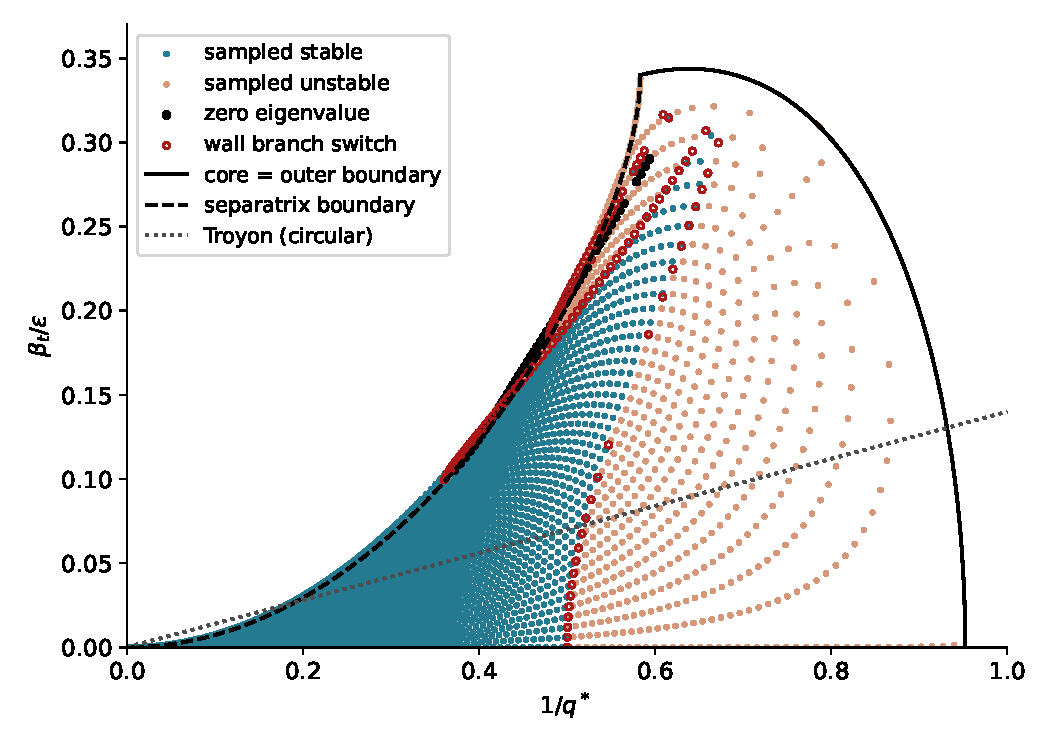
\includegraphics[width=.82\textwidth]{figures/final_stability_space.pdf}\end{center}
图叠两平衡边界, 真零点与分支切换分别标记. 原壁规则在qa\ensuremath{{}^{\prime}}跨整数时会把近壁突然改无穷, 因而部分稳定边界有真实模型跳变, 不能跨跳变求根伪造 $\delta W=0$.

额外薄外环序列逐点检查$m=2,\ldots,16$, 一个实际稳定点为
\begin{align}
 \alpha&=.99999,& \zeta_1&=1.000008513877288,&\nu'&=.8513865575,\\
 q_{a'}&=2.99997788<3,&q_a&=3.00003788,&q_*&=1.57362124,\\
 \beta_t/\epsilon&=.34381640,&\lambda_{\min}&=.6147131\quad(m=2).&&
\end{align}
 该序列一侧趋qa\ensuremath{{}^{\prime}}\ensuremath{\to}3\ensuremath{-}、\ensuremath{\alpha}\ensuremath{\to}1\ensuremath{-}, 候选上确界.34382343、q*1.57360660, 严格端点壁规则变, 所以上确界并非已取到的稳定点. 其远高于题给圆截面Troyon .14/q*\ensuremath{\simeq}.0889676, 差异反映三谐波与等效壁模型, 不是实验反证.

本解完成指定有限空间的实际计算、解析矩阵与扫描, 但不宣称已证明任意m/任意位移和真实全环平衡的全局最高稳定\ensuremath{\beta}. 更多谐波可增负方向, 试探空间正定的量词必须保留. 所有复现代码、扫描、真正零点及壁跳变CSV随源码交付.
\end{solution}
